\documentclass{article}
\usepackage[utf8]{inputenc}
\usepackage[left=1.0cm,right=1.0cm, top=1.5cm, bottom=1.5cm]{geometry}
\usepackage{graphicx}
\usepackage{graphics}
\usepackage{caption}
\usepackage{float}
\usepackage{amsmath}
\usepackage{amssymb}
\usepackage{amsthm}
\usepackage{listings}
\usepackage{mathtools}
\usepackage{hyperref}

% Align all equations left:
\documentclass[fleqn]{article} 


% Sets and quantifiers
\newcommand{\R}{\mathbb{R}\;}
\newcommand{\Q}{\mathbb{Q}\;}
\newcommand{\N}{\mathbb{N}\;}
\newcommand{\nin}{n \in \mathbb{N}}
\newcommand{\fa}{\;\forall\;}
\newcommand{\ex}{\;\exists\;}
\newcommand{\nex}{\;\nexists\;}

% Sequences
\newcommand{\seq}[1]{\{#1\}}
\newcommand{\seqx}{\seq{x_n}}
\newcommand{\seqy}{\seq{y_n}}
\newcommand{\seqs}{\seq{s_n}}

% Subsequences
\newcommand{\seqxni}{\seq{x_{n_i}}}
\newcommand{\seqyni}{\seq{y_{n_i}}}
\newcommand{\xni}{x_{n_i}}
\newcommand{\yni}{y_{n_i}}
\newcommand{\xnij}{x_{n_{i_j}}}
\newcommand{\ynij}{y_{n_{i_j}}}
\newcommand{\seqxnij}{\seq{x_{n_{i_j}}}}
\newcommand{\seqynij}{\seq{y_{n_{i_j}}}}


% Plot functions
\usepackage{tikz}
\usepackage{pgfplots}
\usetikzlibrary{datavisualization}

% Such that
\newcommand{\st}{\;\text{such that}\;}

% Vectors
\newcommand{\xhat}{\hat{\mathbf{x}}}
\newcommand{\yhat}{\hat{\mathbf{y}}}
\newcommand{\zhat}{\hat{\mathbf{z}}}
\newcommand{\nhat}{\hat{\mathbf{n}}}
\newcommand{\shat}{\hat{\mathbf{s}}}
\newcommand{\rhat}{\hat{\mathbf{r}}}
\newcommand{\vhat}{\hat{\mathbf{v}}}
\newcommand{\hatvector}[1]{\hat{\mathbf{1}}}
\newcommand{\mb}[1]{\mathbf{#1}}

% Derivatives
\newcommand{\der}[2]{\frac{d #1}{d #2}}
\newcommand{\dder}[2]{\frac{d^2 #1}{d #2^2}}
\newcommand{\derop}[1]{\frac{d}{d #1}}
\newcommand{\dderop}[1]{\frac{d^2}{d #1^2}}

% Partial Derivatives
\newcommand{\pd}[2]{\frac{\partial #1}{\partial #2}}
\newcommand{\pdd}[2]{\frac{\partial^2 #1}{\partial #2^2}}
\newcommand{\pdop}[1]{\frac{\partial}{\partial #1}}
\newcommand{\pddop}[1]{\frac{\partial^2}{\partial #1^2}}
\newcommand{\pddmixed}[3]{\frac{\partial^2 #1}{\partial #2\partial #3}}
\newcommand{\pddmixedop}[2]{\frac{\partial^2}{\partial #1\partial #2}}

% lim, limsup, liminf
\newcommand{\limn}{\text{lim}_{n \rightarrow \infty}}
\newcommand{\limi}{\text{lim}_{i \rightarrow \infty}}
\newcommand{\limj}{\text{lim}_{j \rightarrow \infty}}
\newcommand{\limsupn}{\limsup_{n \rightarrow \infty}}
\newcommand{\liminfn}{\liminf_{n \rightarrow \infty}}

% Parallel symbols
\newcommand{\parallelsum}{\mathbin{\!/\mkern-5mu/\!}}


% Custom for absolute value
\delimitershortfall-1sp
\newcommand\abs[1]{\left|#1\right|}

% Reference and hyperlink
\newcommand{\source}[1]{\href{#1}{(\textbf{Source})}}

% Use for define equals
\newcommand{\delteq}{\overset{\Delta}{=}}

% For nicer fonts
\usepackage{eucal}

% For Dreamer Paper
\newcommand{\stau}{s_{\tau}}
\newcommand{\expect}[1]{\mathbb{E}_{#1}}
\newcommand{\indep}{\perp \!\!\! \perp}


\title{6.801/6.866: Machine Vision, Lecture 12}
\author{Professor Berthold Horn, Ryan Sander, Tadayuki Yoshitake \\
        MIT Department of Electrical Engineering and Computer Science \\ 
        Fall 2020}
\date{}

\begin{document}

\maketitle
These lecture summaries are designed to be a review of the lecture.  Though I do my best to include all main topics from the lecture, the lectures will have more elaborated explanations than these notes.  Therefore, if you're looking for the most rigorous review and treatment of these topics, we encourage you to rewatch the lecture videos.  With that said, we hope these summaries are beneficial for your learning.  If you have any feedback for these lecture summaries, please submit it \textbf{\href{https://forms.gle/itCUtP4AubAbtwQT9}{here}}.
\section{Lecture 12: Blob Analysis, Binary Image Processing, Use of Green's Theorem, Derivative and Integral as Convolutions
}
In this lecture, we will continue our discussion of intellectual property, and how it relevant for all scientists and engineers.  We will then elaborate on some of the specific machine vision techniques that were used in this patent, as well as introduce some possible extensions that could be applicable for this patent as well.
\subsection{Types of Intellectual Property}
Though it is not related to the technical content of machine vision, being familiar with different types and degrees of intellectual property (IP) is crucial to professional success.  Below, we discuss some of these different types of intellectual property.
\begin{itemize}
    \item \textbf{Patents}: One major type of these is utility and design patents.  In these, the authors are required to disclose the ``best mode" of performance.  For convenience, here are some notes on patents from our previous lecture:
    \begin{itemize}
        \item Can be thought of as a ``contract with society" - you get a limited monopoly on your idea, and in turn, you publish the technical details of your approach.
        \item Can help to reduce litigation and legal fees.
        \item Can be used by large companies as ``ammunition" for ``patent wars".
    \end{itemize}
    Some ``rules" of patents:
    \begin{itemize}
        \item No equations are included in the patent (no longer true)
        \item No greyscale images - only black and white
        \item Arcane grammar is used for legal purposes - ``comprises", ``apparatus", ``method", etc.
        \item References of other patents are often included - sometimes these are added by the patent examiner, rather than the patent authors
        \item Most patents end with something along the lines of ``this is why our invention was necessary" or ``this is the technical gap our invention fills"
        \item Software is not patentable - companies and engineers get around this by putting code on hardware and patenting the ``apparatus" housing the code.
        \item It is also common to include background information (similar to related literature in research).
    \end{itemize}
    \item \textbf{Copyright}:
    \begin{itemize}
        \item Books, song recordings, choreographs
        \item Exceptions: presenting (fractional pieces of) information from another author
    \end{itemize}
    \item \textbf{Trademarks}:
    \begin{itemize}
        \item Must be unique for your field (e.g. Apple vs. Apple).
        \item Cannot use common words - this is actually one reason why many companies have slightly misspelled combinations of common words.
        \item Can use pictures, character distortions, and color as part of the trademark.
        \item No issues if in different fields.
    \end{itemize}
    \item \textbf{Trade Secret}
    \begin{itemize}
        \item No protections, but not spilled, lasts forever
        \item Can enforce legal recourse with Non-Disclosure Agreement (NDA)
    \end{itemize}
\end{itemize}
\subsection{Edge Detection Patent Methodologies}
For this next section, we will direct our attention toward covering concepts that were discussed in the edge detection patent (6,408,109).  Each of these sections will be discussed in further detail below.  Before we get into the specifics of the patent again, it is important to point out the importance of edge detection for higher-level machine vision tasks, such as:
\begin{itemize}
    \item Attitude (pose estimation) of an object
    \item Object recognition
    \item Determining to position
\end{itemize}
We will touch more on these topics in later lectures.
\subsubsection{Finding Edge with Derivatives}
Recall that we find a proposed edge by finding an \textbf{inflection point} of the brightness $E(x,y)$.  The following methods for finding this point are equivalent:
\begin{itemize}
    \item Finding an inflection point of brightness $E(x,y)$.
    \item Finding maximum of brightness gradient magnitude/first derivative $|\nabla E(x,y)|$.
    \item Finding zero crossing of Laplacian/second derivative $\nabla^2 E(x,y)$.
\end{itemize}
For building intuition, last time we used the following example of $u(x) = \sigma(x) = \frac{1}{1 + \exp(-x)}$:
\begin{center}
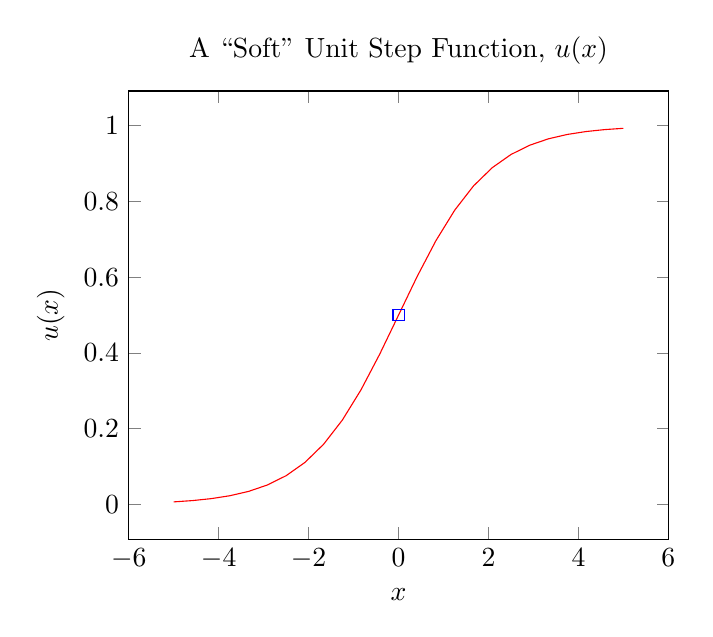
\begin{tikzpicture}
\begin{axis}[
title={A ``Soft" Unit Step Function, $u(x)$},
    xlabel={$x$},
    ylabel={$u(x)$}]
\addplot[color=red]{1/(1 + exp(-x))};
\addplot[
    color=blue,
    mark=square,
    ]
    coordinates {
    (0,0.5)
    };
\end{axis}
\end{tikzpicture}
\end{center}
The gradient of this brightness across the edge, given by $\nabla u(x)$ (or $\der{u}{x}$ in one dimension), is then given by the following.  Notice that the location of the maximum matches the inflection point in the graph above:
\begin{center}
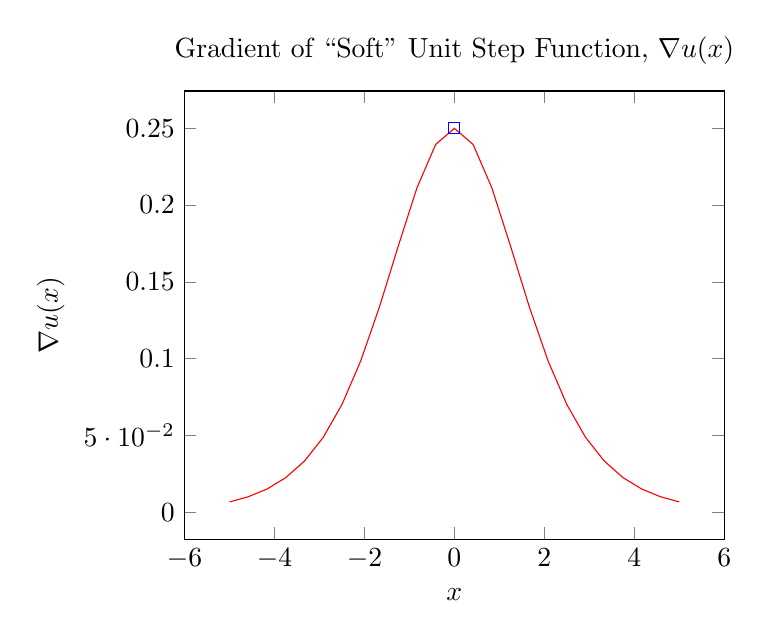
\begin{tikzpicture}
\begin{axis}[
title={Gradient of ``Soft" Unit Step Function, $\nabla u(x)$},
    xlabel={$ x$},
    ylabel={$\nabla u(x)$}]
\addplot[color=red]{exp(-x)/(1 + exp(-x))^2};
\addplot[
    color=blue,
    mark=square,
    ]
    coordinates {
    (0,0.25)
    };
\end{axis}
\end{tikzpicture}
\end{center}
As we mentioned above, we can find the location of this edge by looking at where the second derivative of brightness crosses zero, a.k.a. where $\nabla (\nabla u(x)) = \nabla^2 u(x) = 0$.  Notice that the location of this zero is given by the same location as the inflection point of $u(x)$ and the maximum of $\nabla u(x)$:
\begin{center}
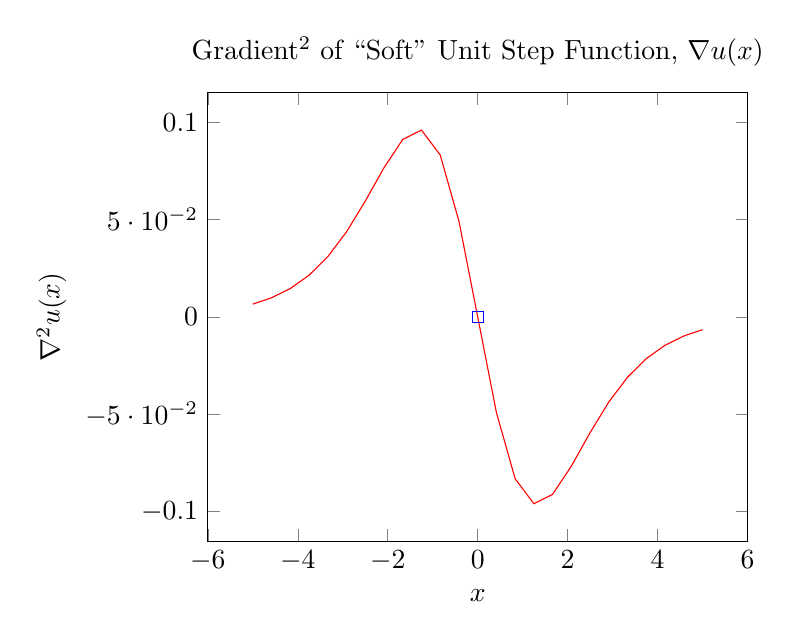
\begin{tikzpicture}
\begin{axis}[
title={Gradient$^2$ of ``Soft" Unit Step Function, $\nabla u(x)$},
    xlabel={$x$},
    ylabel={$\nabla^2 u(x)$}]
\addplot[color=red]{(-exp(-x)*(1+exp(-x))^2 + exp(-x)*2*(1+exp(-x))*exp(-x))/(1+exp(-x))^4};
\addplot[
    color=blue,
    mark=square,
    ]
    coordinates {
    (0,0.0)
    };
\end{axis}
\end{tikzpicture}
\end{center}
For those curious, here is the math behind this specific function, assuming a sigmoid for $u(x)$:
\begin{enumerate}
    \item $u(x) = \frac{1}{1 + \exp{(-x)}}$
    \item $\nabla u(x) = \der{u}{x} = \frac{d}{dx}\Big(\frac{1}{1 + \exp{-x}}\Big) = \frac{\exp(-x)}{(1 + \exp(-x))^2}$
    \item $\nabla^2 u(x) = \dder{u}{x} = \frac{d}{dx}(\frac{\exp(-x)}{(1 + \exp(-x))^2}) = \frac{-\exp(-x)(1+\exp(-x))^2 + 2\exp(-x)(1+\exp(-x))\exp(-x)}{(1+\exp(-x))^4}$
\end{enumerate}
\subsubsection{More on ``Stencils"/Computational Molecules}
Recall that we can use finite differences [1] in the forms of ``stencils" or computational molecules to estimate derivatives in our images.  For this patent, the authors used this framework to estimate the brightness gradient in order to find edges.  For instance, partial derivative of brightness w.r.t. $x$ can be estimated by
\begin{enumerate}
    \item $E_x = \frac{1}{\epsilon}\begin{bmatrix}-1 & 1\end{bmatrix}$
    \item $E_x = \frac{1}{2\epsilon}\begin{bmatrix}-1 & 0 & 1\end{bmatrix}$
    \item $E_x = \frac{1}{2\epsilon}\begin{bmatrix}-1 & 1 \\
                                                    -1 & 1
                                     \end{bmatrix}$
\end{enumerate}
Where for molecule 2, the best point for estimating derivatives lies directly in the center pixel, and for molecules 1 and 3, the best point for estimating derivatives lies halfway between the two pixels. \\ \\
\textbf{How do we analyze the efficacy of this approach}?
\begin{enumerate}
    \item \textbf{Taylor Series}: From previous lectures we saw that we could use averaging to reduce the error terms from 2nd order derivatives to third order derivatives.  This is useful for analytically determining the error.
    \item \textbf{Test functions}: We will touch more on these later, but these are helpful for testing your derivative estimates using analytical expressions, such as polynomial functions.
    \item \textbf{Fourier domain}: This type of analysis is helpful for understanding how these ``stencils"/molecules affect higher (spatial) frequency image content.
\end{enumerate}
Note that derivative estimators can become quite complicated for high-precision estimates of the derivative, even for low-order derivatives.  We can use large estimators over many pixels, but we should be mindful of the following tradeoffs:
\begin{itemize}
    \item We will achieve better noise smoothing/suppression by including more measured values.
    \item Larger derivative estimators linearly (1D)/quadratically (2D) increase the amount of computation time needed.
    \item  Features can also affect each other - e.g. a large edge detection estimator means that we can have two nearby edges affecting each other.
\end{itemize}
We can also look at some derivative estimators for higher-order derivatives.  For 2nd-order derivatives, we just apply another derivative operator, which is equivalent to convolution of another derivative estimator ``molecule":
\begin{align*}
    \pddop{x}(\cdot) = \pdop{x}\Big(\pd{(\cdot)}{x}\Big) \Longleftrightarrow \frac{1}{\epsilon} \begin{bmatrix}-1 & 1\end{bmatrix} \otimes \frac{1}{\epsilon} \begin{bmatrix}-1 & 1\end{bmatrix} = \frac{1}{\epsilon^2}\begin{bmatrix}1 & -2 & 1\end{bmatrix} &&
\end{align*}
For deriving the sign here and understanding why we have symmetry, remember that convolution ``flips" one of the two filters/operators! \\ \\
\textbf{Sanity Check}: Let us apply this to some functions we already know the 2nd derivative of. \\ \\
\begin{itemize}
    \item $f(x) = x^2$:
        \begin{align*}
            f(x) = x^2 \\
            f'(x) = 2x \\
            f''(x) = 2 &&
        \end{align*}
        Applying the 2nd derivative estimator above to this function:
        \begin{align*}
            \begin{bmatrix}1 & -2 & 1\end{bmatrix} \otimes \frac{1}{\epsilon} \begin{bmatrix}f(-1) = 1 & f(0) = 0 & f(1) = 1\end{bmatrix} = \frac{1}{\epsilon^2}((1*1) + (-2*0) + (1*1)) = \frac{1}{\epsilon^2}(1 + 0 + 1) = 1 * 2 = 2 &&
        \end{align*}
        Where we note that $\epsilon = 1$ due to the pixel spacing.  This is equivalent to $f''(x) = 2$.
    \item $f(x) = x$:
        \begin{align*}
            f(x) = x \\
            f'(x) = 1 \\
            f''(x) = 0 &&
        \end{align*}
        Applying the 2nd derivative estimator above to this function:
        \begin{align*}
            \begin{bmatrix}1 & -2 & 1\end{bmatrix} \otimes \frac{1}{\epsilon} \begin{bmatrix}f(-1) = -1 & f(0) = 0 & f(1) = 1\end{bmatrix} = \frac{1}{\epsilon^2}((1*-1) + (-2*0) + (1*1)) = \frac{1}{\epsilon^2}(-1 + 0 + 1) = 0 &&
        \end{align*}
        Where we note that $\epsilon = 1$ due to the pixel spacing.  This is equivalent to $f''(x) = 0$.
    \item $f(x) = 1$:
        \begin{align*}
            f(x) = 1 \\
            f'(x) = 0 \\
            f''(x) = 0 &&
        \end{align*}
        Applying the 2nd derivative estimator above to this function:
        \begin{align*}
            \begin{bmatrix}1 & -2 & 1\end{bmatrix} \otimes \frac{1}{\epsilon} \begin{bmatrix}f(-1) = 1 & f(0) = 1 & f(1) = 1\end{bmatrix} = \frac{1}{\epsilon^2}((1*1) + (-2*1) + (1*1)) = \frac{1}{\epsilon^2}(1 + -2 + 1) = 0 &&
        \end{align*}
        Where we note that $\epsilon = 1$ due to the pixel spacing.  This is equivalent to $f''(x) = 0$.
\end{itemize}
\tetbf{In Practice}: As demonstrated in the example ``test functions" above, in general a good way to test an N$^{\text{th}}$ order derivative estimator is use polynomial test functions of arbitrary coefficients from order 0 up to order N.  For instance, to calculate 4th order derivative estimator, test:
\begin{enumerate}
    \item $f(x) = a$
    \item $f(x) = ax + b$
    \item $f(x) = ax^2 + bx + c$
    \item $f(x) = ax^3 + bx^2 + cx + d$
    \item $f(x) = ax^4 + bx^3 + cx^2 + dx + e$
\end{enumerate}
\textbf{Note}: For derivative estimator operators, the weights of the ``stencils"/computational molecules should add up to zero.  Now that we have looked at some of these operators and modes of analysis in one dimension, let us now look at 2 dimensions.
\subsubsection{Mixed Partial Derivatives in 2D}
First, it is important to look at the linear, shift-invariant property of these operators, which we can express for each quality:
\begin{itemize}
    \item \textbf{Shift-Invariant}: 
    \begin{align*}
        \derop{x}(f(x+\delta)) &= f'(x+\delta), \;\text{for some} \; \delta \in \mathbb{R}\\
        \text{Derivative of shifted function} \;&=\;\text{Derivative equivalently shifted by same amount} &&
    \end{align*}
    \item \textbf{Linear }: 
    \begin{align*}
        \derop{x}(af_1(x) + bf_2(x)) &= af'_1(x) + bf'_2(x) \;\text{for some} \; a,b \in \mathbb{R}\\
        \text{Derivative of scaled sum of two functions} \;&=\;\text{Scaled sum of derivatives of both functions} &&
    \end{align*}
\end{itemize}
We will exploit this \textbf{linear, shift-invariant} property frequently in machine vision.  Because of this joint property, we can treat derivative operators as convolutions in 2D:
\begin{align*}
    \pddmixedop{x}{y}(\cdot) = \pdop{x}\Big(\pdop{y}(\cdot)\Big) \Longleftrightarrow \frac{1}{\epsilon}\begin{bmatrix}-1 & 1\end{bmatrix} \otimes \frac{1}{\epsilon}\begin{bmatrix}1 \\ -1\end{bmatrix} = \frac{1}{\epsilon^2}\begin{bmatrix}-1 & +1 \\ +1 & -1\end{bmatrix} &&
\end{align*}
A few notes here:
\begin{itemize}
    \item The second operator corresponding to $E_y$ has been flipped in accordance with the convolution operator.
    \item If we project this derivative onto a ``diagonal view", we find that it is simply the second derivative of $x'$, where $x'$ is $x$ rotated 45 degrees counterclockwise in the 2D plane: $x' = x\cos 45 + y\cos 45 = \frac{\sqrt{2}}{2}x + \frac{\sqrt{2}}{2}y$. In other words, in this 45-degree rotated coordinate system, $E_{x'x'} = E_{xy}$.
    \item \textbf{Intuition for convolution}: If convolution is a new concept for you, check out reference [2] \href{https://towardsdatascience.com/intuitively-understanding-convolutions-for-deep-learning-1f6f42faee1}{here}.  Visually, convolution is equivalent to ``flipping and sliding" one operator across all possible (complete and partial) overlapping configurations of the filters with one another.
\end{itemize}
\subsubsection{Laplacian Estimators in 2D}
The Laplacian $\nabla^2 \delteq \Delta = \pddop{x} + \pddop{y}$ is another important estimator in machine vision, and, as we discussed last lecture, is the \textbf{lowest-order rotationally-symmetric} derivative operator.  Therefore, our finite difference/computational molecule estimates should reflect this property if they are to be accurate.  Two candidate estimators of this operator are:
\begin{enumerate}
    \item \textbf{``Direct Edge"}: $\frac{1}{\epsilon^2}\begin{bmatrix}0 & 1 & 0 \\
                                                   1 & -4 & 1 \\
                                                   0 & 1 & 0
                                    \end{bmatrix}$
    \item \textbf{``Indirect Edge"}: $\frac{1}{2\epsilon^2}\begin{bmatrix}1 & 0 & 1 \\
                                                     0 & -4 & 0 \\
                                                     1 & 0 & 1
                                    \end{bmatrix}$
\end{enumerate}
Note that the second operator has a factor of $\frac{1}{2\epsilon^2}$ in front of it because the distance between edges is $\sqrt{2}$ rather than 1, therefore, we effectively have $\frac{1}{\epsilon'^2}$, where $\epsilon' = \sqrt{2}\epsilon$. \\ \\
How do we know which of these approximations is better?  We can go back to our analysis tools:
\begin{itemize}
    \item Taylor Series
    \item Test functions
    \item Fourier analysis
\end{itemize}
Intuitively, we know that neither of these estimators will be optimal, because neither of these estimators are rotationally-symmetric.  Let us combine these intelligently to achieve rotational symmetry.  Adding four times the first one with one times the second:
\begin{align*}
    4 \Big(\frac{1}{\epsilon^2}\begin{bmatrix}0 & 1 & 0 \\
                                                   1 & -4 & 1 \\
                                                   0 & 1 & 0
                                    \end{bmatrix}\Big) + 1 \Big(\frac{1}{2\epsilon^2}\begin{bmatrix}1 & 0 & 1 \\
                                                     0 & -4 & 0 \\
                                                     1 & 0 & 1
                                    \end{bmatrix}\Big) = \frac{1}{6\epsilon^2}\begin{bmatrix}1 & 4 & 1 \\
                                                                        4 & -20 & 4 \\
                                                                        1 & 4 & 1
                                                        \end{bmatrix} &&
\end{align*}
Using Taylor Series, we can show that this estimator derived from this linear combination of estimators above results in an error term that is \textbf{one derivative higher} than suing either of the individual estimators above, at the cost of more computation.  Note that the sum of all the entries here is zero, as we expect for derivative estimators. \\ \\
For a hexagonal grid, this is scaled by $\frac{1}{2\epsilon^2}$ and has entries of all 1s on the outer ring, and an entry of -6 in the center.  An example application of a hexagonal grid - imaging black holes!  Leads to $\frac{4}{\pi}$ greater efficiency. \\ \\
As food for thought, what lowest-order rotationally-symmetric \textit{nonlinear} operators?
\begin{align*}
    \sqrt{E^2_{x'} + E^2_{y'}} = \sqrt{E^2_{x} + E^2_{y}} \;\;\text{Where this is the l2 normal of the estimated brightness gradient} &&  
\end{align*}
\subsubsection{Non-Maximum Suppression}
Another technique leveraged in this patent was \textbf{Non-Maximum Suppression (NMS)}.  Idea: Apply edge detector estimator operator everywhere - we will get a small response in most places, so what if we just threshold?  This is an instance of \textbf{early decision-making}, because once we take out these points, they are no longer considered edge candidates in downstream steps. \\ \\
It turns out the authors discourage thresholding, and in their work they remove all but the maximum estimated gradient (note that this is quantized at the octant level).  Note that the quantized gradient direction is perpendicular to the edge.  In this case, for a candidate gradient point $G_0$ and the adjacent pixels $G_{-}$ and $G_{+}$, we must have:
\begin{align*}
    G_0 > G_{-}, G_0 \geq G_{+} &&
\end{align*}
This forces $-\frac{1}{2} \leq s \leq \frac{1}{2}$.
Note that we have the asymmetric inequality signs to break ties arbitrarily.  Next we plot the quantized profile that has been interpolated parabolically - i.e. sub-pixel interpolation.
\subsubsection{Plane Position}
Note that we have not yet done any thresholding.  How can we improve this, given that we quantized the edge gradient direction?  Could we try not quantizing the edge direction?  If we have the true gradient direction, we can find the intersection of this line with the edge (at 90 degrees to the edge gradient) to find a better solution.  \\ \\
To find this point above (please take a look at the handwritten lecture notes for this lecture), we project from the quantized gradient direction to the actual gradient direction.  This is the ``plane position" component.
\subsubsection{Bias Compensation}
Another component of the patent focuses on the interpolation technique used for sub-pixel gradient plotting for peak finding.  To find an optimal interpolation technique, we can plot $s$ vs. $s'$, where $s' = s|2s|^b$, where $b \in \mathbb{N}$ is a parameter that determines the relationship between $s$ and $s'$.  \\ \\
In addition to cubic interpolation, we can also consider piecewise linear interpolation with ``triangle" functions.  For some different values of $b$:
\begin{itemize}
    \item $b = 0 \rightarrow s' = s$
    \item $b = 1 \rightarrow s' = 2\;\text{sign}(s)s^2$
    \item $b = 2 \rightarrow s' = 4\;\text{sign}(s)s^3$
\end{itemize}
Where different interpolation methods give us different values of $b$.
\subsubsection{Edge Transition and Defocusing Compensation}
Another point of motivation: most edge detection results depend on the actual edge transition.   Why are edges fuzzy (note that some degree of fuzziness is needed to prevent aliasing)?  One major cause of fuzziness is ``defocusing", in which the image plane and ``in focus" planes are slightly off from one another.  This causes a ``pillbox" of radius $R$ to be imaged (see handwritten lecture notes), rather than the ideal case of an impulse function $\delta(x,y)$.  This radius is determined by:
\begin{align*}
    R = \delta\frac{d^2}{f} \;(\textbf{Point Spread Function (PSF)}) &&
\end{align*}
This pillbox image is given mathematically by:
\begin{align*}
    \frac{1}{\pi R^2}(1 - u(r-R)) &&
\end{align*}
Where $u(\cdot)$ is the unit step function.
Where $f$ is the focal length of the lens, $d$ is the diameter of the lens (assumed to be conic), and $\delta$ is the distance along the optical axis between the actual image plane and the ``in focus" plane.
\subsection{Multiscale}
\textbf{Note}: We will discuss this in greater detail next lecture. \\ \\
Multiscale is quite important in edge detection, because we can have edges at different scales.  To draw contrasting examples, we could have an image such that:
\begin{itemize}
    \item We have very sharp edges that transition over $\approx$ only 1 pixel
    \item We have blurry edges that transition over many pixels
\end{itemize}
\subsubsection{Effect on Image Edge}
Here is one possible extension not included in the edge detection patent. \\ \\
We can slide a circle across a binary image - the overlapping regions inside the circle between the 1-0 edge controls how bright things appear.  We can use this technique to see how accurately the algorithm plots the edge position - this allows for error calculation since we have ground truth results that we can compute using the area of the circle.  Our area of interest is given by the area enclosed by the chord whose radial points intersect with the binary edge:
\begin{align*}
    & A = R^2\theta - \frac{2\sqrt{R^2-X^2}X}{2} \\
    & \theta = \arctan\Big(\frac{\sqrt{R^2-x^2}}{x}\Big) &&
\end{align*}
Another way to analyze this is to compute the analytical derivatives of this brightness function:
\begin{enumerate}
    \item $\pd{E}{x} = 2\sqrt{R^2 - x^2}$
    \item $\pdd{E}{x} = \frac{-2x}{\sqrt{R^2 - x^2}}$
\end{enumerate}
What can we do with this?  We can use this as input into our algorithm to compute teh error and \textbf{compensate} for the degree of defocusing of the lens.  In practice, there are other factors that lead to fuzzy edge profiles aside from defocusing, but this defocusing compensation helps.
\subsubsection{Addressing Quantization of Gradient Directions}
Here is another possible extension not included in the edge detection patent. \\ \\
Recall that because spaces occurs in two sizes (pixel spacing and $\sqrt{2}$ pixel spacing), we need to sample in two ways, which can lead to slightly different error contributions.  We do not want quantized gradient directions.  To do this, we can just interpolate values $G_{-}, G_0, G_{+}$ along the true edge gradient!  \\ \\
\textbf{Linear 1D Interpolation}: 
\begin{align*}
    \tilde{f}(x) = \frac{f(a)(b-x) + f(b)(x-a)}{b-a} &&
\end{align*}
We can also leverage more sophisticated interpolation methods, such as \textbf{cubic spline}. \\ \\
\textbf{Why did the authors not leverage this interpolation strategy?}
\begin{itemize}
    \item this requires the spacing of any level, i.e. not just pixel and $\sqrt{2}$ pixel spacing, but everything in between.
    \item Since you interpolate, you are not using measured values.  Introduces some uncertainty that may be too much to achieve 1/40$\text{th}$ pixel accuracy.
\end{itemize}
What can we do to address this?  $\rightarrow$ \textbf{Project gradient onto unit circle!}  This requires 2D interpolation, which can be done with methods such as bilinear or bicubic interpolation.
\subsubsection{CORDIC}
As we discussed in the previous lecture, CORDIC is an algorithm used to estimate vector direction by iteratively rotating a vector into a correct angle.  For this patent, we are interested in using CORDIC to perform a change of coordinates from cartesian to polar:
\begin{align*}
    (E_x, E_y) \rightarrow (E_0, E_{\theta}) &&
\end{align*}
\textbf{Idea}: Rotate a coordinate system to make estimates using test angles iteratively.  Note that we can simply compute these with square roots and arc tangents, but these can be prohibitively computationally-expensive:
\begin{align*}
    & E_0 = \sqrt{E^2_x + E^2_y} \\
    & E_{\theta} = \arctan\Big(\frac{E_y}{E_x}\Big) &&
\end{align*}
Rather than computing these directly, it is faster to iteratively solve for the desired rotation $\theta$ by taking a sequence of iterative rotations $\{\theta_i\}_{i=1, 2, \cdots}^{n}$.  The iterative updates we have for this are, in matrix-vector form:
\begin{align*}
    \begin{bmatrix}E^{(i+1)}_x \\ E^{(i+1)}_y \end{bmatrix} & = \begin{bmatrix}\cos\theta_i & \sin\theta_i \\ -\sin\theta_i & \cos\theta_i\end{bmatrix}\begin{bmatrix}E^{(i)}_x \\ E^{(i)}_y \end{bmatrix} \\
    \text{Gradients at next step} & = \;\text{Rotation R by} \; \theta_i \times \;\text{Gradients at current step} &&
\end{align*}
How do we select $\{\theta_i\}_{i=1, 2, \cdots}^{n}$?  We can select progressively smaller angles.  We can accept the candidate angle and invoke the iterative update above if each time the candidate angle reduces $|E_y|$ and increases $|E_x|$. \\ \\
The aggregate rotation $\theta$ is simply the sum of all these accepted angles: $\theta = \sum_{i}\theta_i$ \\ \\
One potential practical issue with this approach is that it involves a significant number of multiplications.  How can we avoid this?  We can pick the angles carefully - i.e. if our angles are given successively by $\frac{\pi}{2}$, $\frac{\pi}{4}$, $\frac{\pi}{8}$, ..., then:
\begin{align*}
    \frac{\sin\theta_u}{\cos\theta_i} = \frac{1}{2^i} \rightarrow \;\text{rotation matrix becomes}: \; \frac{1}{\cos\theta_i}\begin{bmatrix}1 & 2^{-i} \\ -2^{-i} & 1\end{bmatrix} &&
\end{align*}
Note that this reduces computation to 2 additions per iteration.  Angle we turn through becomes successively smaller:
\begin{align*}
    \cos\theta_i = \sqrt{1 + \frac{1}{2^{2i}}} \rightarrow R = \prod_{i}\cos\theta_i = \prod_{i}\sqrt{1 + \frac{1}{2^{2i}}} \approx 1.16 \;(\text{precomputed}) &&
\end{align*}

\subsection{References}
\begin{enumerate}
    \item Finite Differences, https://en.wikipedia.org/wiki/Finite\_difference
    \item Convolution, https://towardsdatascience.com/intuitively-understanding-convolutions-for-deep-learning-1f6f42faee1
\end{enumerate}
\end{document} 

